
\section{Introduction}
\label{chap:introduction}

The mission of the first edition of this book (2012) was to introduce
the anykernel and rump kernels and motivate their existence.  Additionally, we explored
the characteristics of the technology through various experiments.
The paramount, often criminally overlooked experiment was the one hiding in
plain sight: is it possible to construct the system in a sustainable,
real-world compatible fashion.  That paramount experiment was shown
to be a success, and that result has not changed since the original
publication, only strengthened.  The core technology is still almost
identical to the one described in the original book.

This new edition has been written to account for the practical experiences
from new use cases, many of which were proposed in the first edition,
but which have since become reality.

To start off, we will look at operating systems in general: what one is,
how they developed throughout history, where they are now, what the
problem is, and why the time is now ripe for change.  After that, we
will briefly introduce the Anykernel and Rump Kernels, and argue why
they are part of the solution to the problem.


\subsection{Operating Systems}

The term \textit{operating system} originally meant a system which aids
computer operators in loading tapes and punchcards onto the
computer~\cite{dijkstra:ewd1303}.  We take a slightly more modern
approach, and define an operating system as a collection
of subroutines which allow application programs to run on a given
\textit{platform}.  The platform can be for example a physical unit of
hardware, or be virtually provisioned such as on the cloud.  Additionally,
an operating system may, for example, multiplex the platform for a number
of applications, protect applications from each other, be distributed
in nature, or provide an interface which is visually appealing to
some people.

The majority of the operating system is made up of \textit{drivers},
which abstract some underlying entity.  For example, device drivers
know which device registers to read and write for the desired result,
file system drivers know which blocks contain which parts of which files,
and so forth.  In essence, a driver is a \textit{protocol translator},
which transforms requests and responses to different representations.

There is nothing about protocol translation which dictates that a driver
must be an integral part of an operating system as opposed to being part
of application code.  However, operating system drivers may also be used
as a tool for imposing protection boundaries.  For example, an operating
system may require that applications access a storage device through
the file system driver.  The file system can then enforce that users
are reading or writing only the storage blocks that they are supposed to
have access to.  As we shall see shortly, imposing privilege boundaries
grew out of historic necessity when computers were few and the operating
system was a tool to multiplex a single machine for many users.


\subsubsection{Historical Perspective}

Computers were expensive in the 1950's and 1960's.  For example, the cost of
the UNIVAC I in 1951 was just short of a million dollars.  Accounting for
inflation, that is approximately 9 million dollars in today's money.
Since it was desirable to keep expensive machines doing something
besides idling, batch scheduling was used to feed new computations and
keep idletime to a minimum.

As most of us intuitively know, reaching the solution of a problem is
easier if you are allowed to stumble around with constant feedback, as
compared to a situation where you must have holistic clairvoyance over the
entire scenario before you even start.  The lack of near-instant feedback
was a problem with batch systems.  You submitted a job, context switched
to something else, came back the next day, context switched back to your
computation, and discovered your program was missing a comma.

To address the feedback problem, timesharing was invented.  Users logged
into a machine via a terminal and got the illusion of having the whole
system to themselves.  The timesharing operating system juggled between
users and programs.  Thereby, poetic justice was administered: the
computer was now the one context-switching, not the human.  Going from
running one program at a time to running multiple at the ``same'' time
required more complex control infrastructure.  The system had to deal
with issues such as hauling programs in and out of memory depending on
if they were running or not (swapping), scheduling the tasks according
to some notion of fairness, and providing users with private, permanent
storage (file system).  In other words, 50 years ago they had the key
concepts of current operating systems figured out.  What has happened
since?

\subsubsection{And Where It Got Us}

The early timesharing systems isolated users from other users.
The average general purpose operating system still does a decent job at
isolating users from each other.  However, that type of isolation does
little good in a world which does not revolve around people logging
into a timesharing system.  The increasing problem is
isolating the user from herself or himself.  Ages ago, when you yourself
wrote all of the programs you ran, or at least had a physical interaction
possibility with the people who did, you could be reasonably certain
that a program you ran did not try to steal your credit card numbers.
These days, when you download a million lines of so-so trusted application
code from the Internet, you have no idea of what happens when you run
it on a traditional operating system.

The timesharing system also isolates the system and hardware components
from the unprivileged user.  In this age when everyone has their own
hardware --- virtual if not physical --- that isolation vector is of
questionable value.  It is no longer a catastrophe if an unprivileged
process binds to transport layer ports less than 1024.  Everyone should
consider reading and writing the network medium unlimited due to
hardware no longer costing a million, regardless of what the operating
system on some system does.  The case for separate system and user
software components is therefore no longer universal.  Furthermore,
the abstract interfaces which hide underlying power, especially that of
modern I/O hardware, are insufficient for high-performance
computing~\cite{peter:arrakis}.

In other words, since the operating system does not protect the user
from evil or provide powerful abstractions, it fails its mission
in the modern world.  Why do we keep on using such systems?  Let us
imagine the world of computing as a shape sorter.  In the beginning,
all holes were square: all computation was done on a million dollar
machine sitting inside of a mountain.  Square pegs were devised to fit
the square holes, as one would logically expect.  The advent of timesharing brought better square pegs, but
it did so in the confines of the old scenario of the mountain-machine.
Then the world of computing diversified.  We got personal computing,
we got mobile devices, we got IoT, we got the cloud.  Suddenly, we had
round holes, triangular holes and the occasional trapezoid and rhombus.
Yet, we are still fascinated by square-shaped pegs, and desperately try
to cram them into every hole, regardless of if they fit or not.

Why are we so fascinated with square-shaped pegs?  What happens if we
throw away the entire operating system?  The first problem with that
approach is, and it is a literal show-stopper, that applications will
fail to run.  Already in the late 1940's computations used subroutine
libraries~\cite{campbell-kelly:edsac}.  The use of subroutine libraries
has not diminished in the past 70 years, quite to the contrary.
An incredible amount of application software keeping the Internet and the
world running has been written against the POSIX-y interfaces offered
by a selection of operating systems.  No matter how much you do not
need the obsolete features provided by the square peg operating system,
you do want to keep your applications working.

From-scratch implementations of the services provided by operating systems
are far from trivial undertakings.  Just implementing the 20-or-so flags
for the \texttt{open()} call in a real-world-bug-compatible way is far
from trivial.  Assuming you want to run an existing libc/application
stack, you have to keep in mind that you still have roughly 199 system
calls to go after \texttt{open()}.  After you are done with the system
calls, you then have to implement the actual components that the system
calls act as an interface to: networking, file systems, device drivers,
and various other driver stacks.

After the completing the above steps for a from-scratch implementation,
the most time-consuming part remains: \textit{testing your implementation
in the real world and fixing it to work there}.  This step is also the
most difficult one, since no amount of conformance to formal specification
or testing in a laboratory is a substitute for being ``bug-compatible''
with the real world.

So in essence, we are fascinated by square-shaped pegs because our
applications rest on the support provided by those pegs.  That is why
we are stuck in a rut and few remember to look at the map.


\subsubsection{What We Really Need}

We want applications to run.  We need the operating system to
adapt to the scenario the application is deployed in, not for the
application to adapt to a 1950's understanding of computing and hardware
cost.

Let us consider embedded systems.  Your system consists of one trust-domain on one piece
of hardware.  There, you simply need at set of subroutines (drivers) to
enable your application to run.  You do not need any code which allows
the single-user, single-application system to act like a timesharing
system with multiple users.  However, for example the implementation
of the TCP/IP driver can, assuming you do not want to scale to
kilobyte-sized system or to the bleeding edge of performance, be the
same as one for a multiuser system.  After all, the TCP/IP protocols
are standard, and therefore the protocol translation the driver needs
to perform is also standard.

Let us consider the cloud and especially microservices running on the cloud.
We can indeed run the services on top of a timesharing operating system,
A paravirtualized timesharing OS takes time to bootstrap~\cite{jiang:soda}
and consumes resources even for the features which are not used by
the microservice.  OS virtualization via containers~\cite{phk:jails}
provides better performance and resource consumption than
paravirtualization~\cite{soltesz:containers,wang:overhead}, but at the
cost of putting millions of lines of code into the trusted computing base.

Using timesharing systems en masse will allow applications to run in both
cases, but not adapting to the scenario comes with a price.  In effect,
tradeoffs are made either for performance or security.


\subsection{The Anykernel and Rump Kernels}

This work is about how to move from the world of timesharing systems
to the world of the future in a fashion in which applications continue
to function.  The two key terms are \textit{anykernel} and
\textit{rump kernel}, both of which we will introduce and describe shortly.

Applications need subroutines to work, and those subroutines are provided
by operating systems.  We call those subroutines drivers, and state that
not only does a typical application require a large set of drivers,
but also that those drivers are also non-trivial to write and maintain.  While
operating systems built around a timesharing model are rich in drivers
due to having a lot of history behind them, they are not sufficient for
the use cases required by the modern world.  We need to
start treating drivers as library-like components instead of requiring a
separate implementation for each operating system.  The library-approach
will allow to build the software stack to suit the scenario, instead of
having to build the scenario to suit the available operating systems.

The term \textit{anykernel} was coined in response to the ever-increasing
number of operating system models: monolithic kernel, microkernel,
exokernel, multikernel, unikernel, etc.  As the saying goes,
creating something new is is 5\% inspiration and 95\% perspiration.
While the inspiration required to come up with a new model should not be
undervalued, after that 95\% of the work for reaching a usable software
stack remains.  That 95\% consists largely of the drivers.  For example,
even the most trivial cloud operating system requires a TCP/IP driver,
and creating one from scratch or even porting one is far from trivial.
The anykernel is a term describing a kernel-type codebase from which
drivers, the 95\%, can be extracted and integrated to \textit{any}
operating system model --- or at least near any --- without porting and
maintenance work.

A \textit{rump kernel}, as the name implies, is a timesharing style
kernel from which portions have been removed.  What remains are drivers
and the basic support routines required for the drivers to function --
synchronization, memory allocators, and so forth.  What is gone are
policies of thread scheduling, virtual memory, application processes,
and so forth.  Rump kernels have a well-defined (and small!) portability
layer, so they are straightforward to integrate into various environments.

\begin{figure}[t]
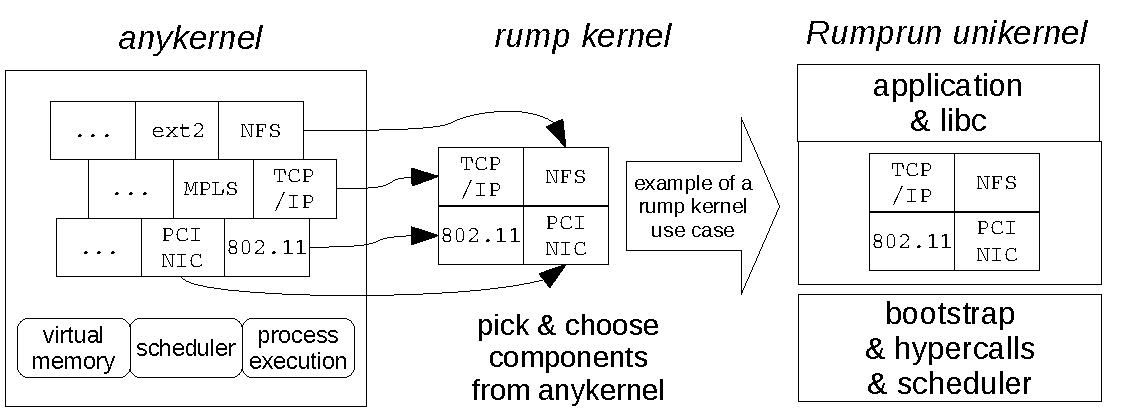
\includegraphics[width=\linewidth]{imgs/concept-comparison}
\caption[Relationship between key concepts]
{\textbf{Relationship between key concepts}:
The anykernel allows driver components to be lifted out of the original
source tree and rump kernels to be formed out of those drivers.
Rump kernels can be used to build products and platforms; one example
of a use case is illustrated.
}
\label{fig:concept-comparison}
\end{figure}

Figure~\ref{fig:concept-comparison} illustrates how a timesharing system,
anykernel and rump kernel are related.  The figure indeed illustrates
only one example, and by extension, only one example platform for hosting
rump kernels.

Throughout most of the technical discussion in this book we will
consider a userspace program as the platform for hosting a rump kernel.
There are two reasons why it is so.  First, the original motivation for
rump kernels back in 2007 was developing, debugging and testing kernel
drivers.  What better place to do it than in userspace?  Second, userspace
is in itself a ``hosted'' platform, and we do not have full control of
for example the symbol namespace or the scheduler.  Therefore, if rump
kernels can work in userspace, they can also easily work on platforms
which are custom-built to host rump kernels.

The implementation we discuss is available in NetBSD.  It is crucial
to differentiate between the implementation being \textit{in} NetBSD,
and it being available as patches for NetBSD.  The idea of the anykernel
is that it is an inherent property of a code base, so as to keep things
maintained.  What, in fact, keeps the implementation working is NetBSD's
internal use of rump kernels for testing kernel drivers.  This testing
also allows NetBSD to provide better quality drivers, so there is clear
synergy.  However, we will not focus on the testing aspects in this book;
if curious, see the first edition for more discussion on development
and testing.


\subsection{Book Outline}

The remainder of the book is as follows.  \chapref{concept} defines the
concept of the anykernel and rump kernels and \chapref{implementation}
discusses the implementation and provides microbenchmarks as supporting
evidence for implementation decisions.  Essentially, the two previous
chapters are a two-pass flight over the core subject.  The intent is to
give the reader a soft landing by first introducing the new concept in
abstract terms, and then doing the same in terms of the implementation.
That way, we can include discussion of worthwhile implementation details
without confusing the high-level picture.  If something is not clear from
either chapter alone, the recommendation is to study the relevant text from
the other one.  If you read the first edition of this book, you may choose
to only lightly skim these two chapters; the main ideas are the same
as in the first edition.

\chapref{ecosystem} gives an overview of what we have
built on top of rump kernels.  A brief history of the project is
presented in \chapref{history}.  The history chapter can be read first,
last, or anywhere in between, or not at all.  Finally,
\chapref{conclusions} provides concluding remarks.


\subsubsection*{What this book is not}

This book is not a user manual.  You will not learn how to use rump
kernels in day-to-day operations from this book.  However, you will gain a
deep understanding of rump kernels which, when coupled with the user
documentation, will give you superior knowledge of how to use rump
kernels.  Most of the user documentation is available as a wiki at
\url{http://wiki.rumpkernel.org/}.


\subsection{Further Material}

In general, further material is reachable from the rump kernel
project website at \url{http://rumpkernel.org/}.

\subsubsection{Source Code}
\label{sect:src}

The NetBSD source files and their respective development histories are
available for study from repository provided by the NetBSD project,
\eg via the web interface at \texttt{cvsweb.NetBSD.org}.  These files
are most relevant for the discussion in \chapref{concept} and
\chapref{implementation}.

The easiest way to fetch the latest NetBSD source code in bulk is to
run the following commands (see Section~\ref{sect:srcnetbsd} for further
information):

\begin{verbatim}
git clone http://repo.rumpkernel.org/src-netbsd
cd src-netbsd
git checkout all-src
\end{verbatim}

Additionally, there is infrastructure to support building rump kernels
for various platforms hosted at \url{http://repo.rumpkernel.org/}.
The discussion in \chapref{ecosystem} is mostly centered around
source code available from that location.

\subsubsection*{Code examples}

This book includes code examples from the NetBSD source
tree.  All such examples are copyright of their respective owners
and are not public domain.  If pertinent, please check the full
source for further information about the licensing and copyright
of each such example.

\subsubsection{Manual Pages}

Various manual pages are cited in the document.  They are available
as part of the NetBSD distribution, or via the web interface
at \url{http://man.NetBSD.org/}.
